\documentclass{article}

\usepackage{graphicx}

\begin{document}

\begin{titlepage}
\title{Searching for circuit complexity lower bounds using SAT solvers}
\author{August Taylor}
\maketitle
\end{titlepage}

\begin{abstract}
Where the abstract will go
\end{abstract}

\tableofcontents

\section{Introduction}

\subsection{Motivation}

Finding lower bounds on the size of Boolean circuits computing given Boolean functions is one of the most fundamental open problems in computer science. Despite the fact that the majority of functions have exponential circuits, the best lower bounds proven on unrestricted circuits are only linear~\cite{boppana} and we still do not have optimal circuits or close upper and lower bounds for many important functions. Results in this area can be used to separate computational complexity classes, possibly even P and NP (i.e. to show that a large class of fundamental and practically useful problems do not have polynomially fast algorithms).~\cite{arora} 

If functions with circuits of a given complexity could be identified by an efficient algorithm, this could be used to construct efficient learning algorithms for circuits of a smaller complexity.~\cite{carmosino} Furthermore, such an algorithm could be used to break pseudorandom generators (i.e. distinguish random from pseudorandom inputs), which would have major implications in the field of cryptography.~\cite{arora}

A heuristic approach is to find minimal circuits for small instances of the functions. This can be used to prove new bounds~\cite{kulikovsurvey} and may lead to theoretical insights on the structure of their optimal circuits generally~\cite{williams}. Finding efficient circuits is also necessary in practice when designing electronic systems. 

One approach to automating the search for efficient circuits is to reduce the problem of designing a correct circuit (logical design synthesis) to the Boolean satisfiability problem (SAT). Existing algorithms (SAT solvers) can then be used to solve the problem, either finding a correct circuit of fixed size or generating a proof that none exists~\cite{kulikov}.

\subsection{Previous work}

Kamath et al~\cite{kamath} propose a reduction from logical design synthesis to SAT which fixes the DNF structure of the circuit and number of disjunctions used. Experiments using this reduction to find minimal circuits for 2-4 bit adders and multipliers are reported in~\cite{estrada}. Kojevnikov et al~\cite{kulikov} demonstrate a more general reduction allowing any circuit with a fixed number of gates, proving linear bounds for \(MOD^n_3\) circuits over different Boolean bases. This was done by checking for circuit 'building blocks' with 5 to 11 gates. In~\cite{kulikovlocal} the same reduction was used to improve large circuit building blocks by searching for smaller versions of their sub-circuits. Specifically, linear upper bounds were proved or verified for \(SUM\), \(MOD^n_4\), and \(MOD^n_3\) by checking for circuits with up to 13 gates.

*Mention valiant universal circuits?

*Should look for other things

\subsection{Our contributions}

We investigate feasible ways to find small circuits using SAT reductions. Previous research in this area has focused on a small number of target Boolean functions and a single reduction at a time. Instead we use multiple combinations of reductions and SAT solvers to see which leads to the best performance, testing them on a range of different functions. 

We also present a new reduction *not sure what to say about this*

*Extension axioms - should actually try them first


\section{Background}

\subsection{General setting}

Denote by \(B_{n,m}\) the set of all Boolean functions \(f: \{0,1\}^n \to \{0,1\}^m\) and let \(B_n = B_{n,1}\). A circuit over the basis \(A \subseteq B_2\) is a directed acyclic graph with nodes of in-degree 0 or 2. Nodes of in-degree 0 are called inputs. Nodes of in-degree 2 are assigned functions from \(A\) and are called gates. Some nodes may be also be marked as outputs.

Without loss of generality, we can also assert that every gate has a larger index than both of its predecessors (i.e. the gates are sorted topologically w.r.t. the used numbering); that every gate's second predecessor has a larger index than its first predecessor; and that the last gate is an output.~\cite{kulikov}

A circuit \(c\) of size N is said to compute the function \(f\in B_{n,m}\) if, for all input vectors \(v\in\{0,1\}^n\) in the range of \(f\), \(c(v)=f(v)\), where \(c(v) = (o_1,...o_m)\) are the values of the output gates of \(c\), each input \(x_i\) takes value \(v_i\), and each gate takes the value of its assigned function when applied to the value of its two predecessor nodes.

In this paper, we mainly consider circuits over the De Morgan basis \[C_2 = \{\lor, \land, \neg\}\] where \(\neg\) denotes the Boolean function which outputs the negation of its first argument.

The size of a circuit is its number of gates. We define the circuit existence problem as the question of whether, given a truth table for a function \(f: \{0,1\}^n \to \{0,1\}^m\), there exists a circuit of size N computing \(f\).

\subsection{Reduction to SAT}

We encoded the circuit existence problem as a Boolean formula using three reductions.

\subsubsection{Existing reductions}

The first is due to Kojevnikov et al~\cite{kulikov} who present it together with bounds on the growth rate of the formula. The basis of the circuit can be specified as any subset of \(B_2\). The number of clauses generated is \(O(N^3\cdot2^n)\) and the number of variables is \(O(2^n\cdot N)\)

The second is due to Razborov~\cite{raz} and requires a circuit over the basis \(C_2\): *not sure how much to describe this one but I definitely need to give the growth rates..*

*Also am bothered that this is the only reduction that allows constants in the circuit - it wouldn't be hard to remove that aspect.*

\subsubsection{A new reduction}

The third reduction is straightforward and also requires a circuit over the basis \(C_2\).

It uses the following variables:

\begin{enumerate}
  \item \(e^i_a\) \((n \leq i < N, a\in\{0,1\}^n)\) is the value of the \(i\)-th gate when the input to the circuit is \(a\). It gives \(O(N\cdot 2^n)\) variables.
  \item \(x_{i,j}\) \(( 0 \leq i < N+n,0 \leq j < i)\) is true iff j is a predecessor of i. It gives \(O(N\cdot (N+n))\) variables.
  \item \(g^0_i, g^1_i\) \((n \leq i < N)\) together encode the function assigned to the \(i\)-th gate by their truth values, giving \(2N\) variables:

    \begin{center}
    \begin{tabular}{ |c|c|c| }
    \hline
    \(g^0_i\) & \(g^1_i\) & Function \\ 
    \hline
    0 & 0 & \(\neg\) \\  
    0 & 1 & \(\lor\) \\ 
    1 & 0 & \(\land\) \\ 
    1 & 1 & \(\neg\) \\   
    \hline
    \end{tabular}
    \end{center}

\end{enumerate}

We encode the requirements for the circuit by the following clauses:

\begin{enumerate}
  \item For all \((i,j,k)\) with \(n \leq i < n+N\), \(0 \leq j < i\) and \(j < k < i\), and for all \(a\in\{0,1\}^n\), if \(j\) and \(k\) are both predecessors of \(i\), then \(e^i_a\) must take the value computed by the \(i\)th gate's assigned function on \(e^j_a\) and \(e^k_a\). A clause must be added for each function in the basis. For example, the clause for when the \(i\)th gate is an \(\land\)-gate:

\[
(g^0_i\wedge \neg g^1_i)\wedge 
(x_{i,j}\wedge x_{i,k})\rightarrow 
(e^i_a\leftrightarrow e^j_a\wedge e^k_a)
\]
  
  Note that the gate must compute the conjunction of any two predecessors' variables. This means it can have at most two predecessors, otherwise the conjunctions of different pairs of predecessors may disagree and the gate will have no correct value. This leads to \(O(2^n\cdot N^3)\) 7-clauses.

  \item For all \(i\) with \(n \leq i < n+N\), gate \(i\) must have at least one predecessor. This leads to \(O(N)\) \(O(N+n)\)-clauses.

  \item For all \((i,j)\) with \(n \leq i < n+N\), \(0 \leq j < i\), if \(i\) is an \(\lor\)-gate or \(\land\)-gate with \(j\) its predecessor, it must have another distinct predecessor (i.e. it must have at least 2 overall). For example, the clause for when the \(i\)th gate is an \(\land\)-gate:

\[
(g^0_i \land \neg g^1_i) \rightarrow \left( x_{i,j} \rightarrow \bigvee_{j<k<i} x_{i,k} \right)
\]

  This leads to \(O(N^2)\) \(O(N)\)-clauses.

  \item For all \(i\) with \(0 \leq i < n\), \(a\in\{0,1\}^n\), the \(i\)-th input must equal \(a_i\). This leads to \(O(n \cdot 2^n)\) 1-clauses.

  \item For all \(a\in\{0,1\}^n\), the final m gates (i.e. the outputs) should agree with the output values given for \(a\) in the target truth table. This leads to \(O(2^n)\) 1-clauses.

\end{enumerate}

\subsection{Extension axioms}

\section{Results}

Timed experiments were carried out on a 3.400GHz Intel i3-8130U processor running Linux. The times shown were obtained by running the software on the problem 3 times and taking the mean.

We chose to investigate the existence of circuits up to 9 gates, as these were reliably solved within less than 12 hours on the hardware described.

\subsection{Comparison of Boolean functions}

We investigated the relationship between the size of a circuit and the time taken for a SAT solver to confirm or deny its existence. We encoded a range of simple symmetric functions using the Kulikov encoding *define them more clearly:

\begin{enumerate}
  \item AND on 7 and 8-bit inputs
  \item Parity on 3- and 4-bit inputs
  \item \(MOD^0_3\) and \(MOD^0_4\) on 3- and 4-bit inputs
  \item Majority on 3 and 4-bit inputs
  \item Partial parity - Explain why partial functions are useful for encoding lower bounds on big input-lengths. But also need to find a way to get good data for them (ie. more than 1 second per problem...)

\end{enumerate}

\begin{figure}[!ht]
%  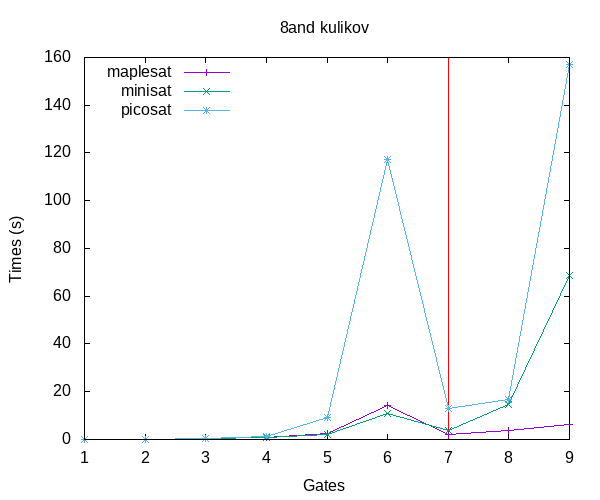
\includegraphics[width=\textwidth]{images/times/8and kulikov.png}
\end{figure}
The size of the minimal circuit is shown in red. It was found that the time needed tended to spike on or around the optimal circuit size. This may be because it is difficult to confirm or rule out circuits that come close to satisfying the requirements. A similar phenomenon was reported in~\cite{estrada}.

A complete display of graphs can be found in the appendix.

\subsection{Comparison of SAT solvers and reductions}

We used three SAT solvers, each based on DPLL with a variety of heuristics. (give a brief introduction on minisat, picosat, maplesat)

We investigated whether there was a relationship between the reduction used to encode a Boolean function, the solver used, and the time taken by the solver.

\begin{figure}[!ht]
  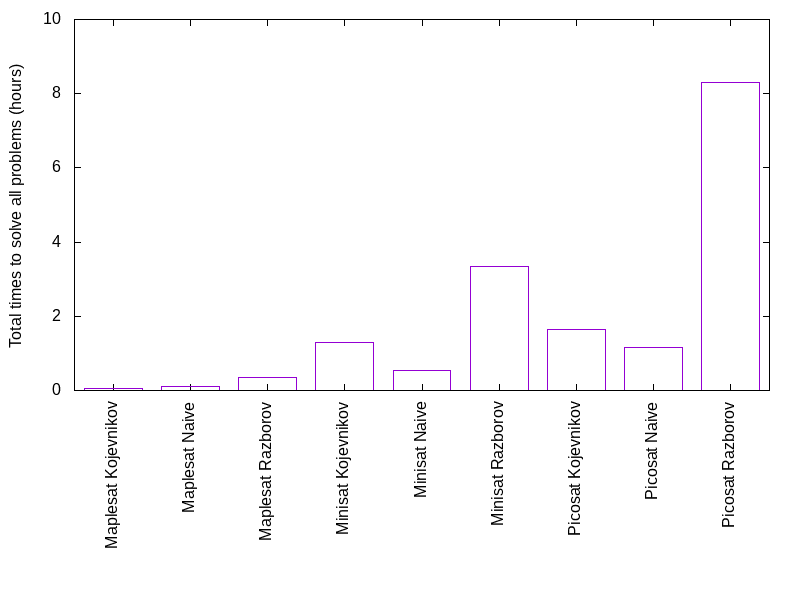
\includegraphics[width=\textwidth]{images/totals.png}
  \label{fig:totals}
  \caption{Comparison of times taken by SAT solvers on different reductions}

\end{figure}

It can be seen that MapleSAT on the Kulikov encoding performs the best. Apart from this, the effect of the reduction and the solver seem to be independent, with MapleSAT consistently performing better than MiniSAT and PicoSAT, and the naive and Kulikov reductions performing better than the Razborov reduction. **however I should take out the constants and re-run the experiments to be sure it’s not that..

\subsection{Random functions}

16 truth tables were generated for 3 and 4-bit inputs using a pseudorandom number generator (specifically, xorshift128+ due to the Javascript implementation) simulating a uniform distribution. The tables were encoded with the Kulikov reduction and solved using MapleSAT. The times taken to check for circuits of different sizes are shown in

*images*

The distribution of minimal circuit sizes needed to implement these functions are shown in \ref{fig:3rand_sizes} and \ref{fig:4rand_sizes}.

\begin{figure}[!ht]
  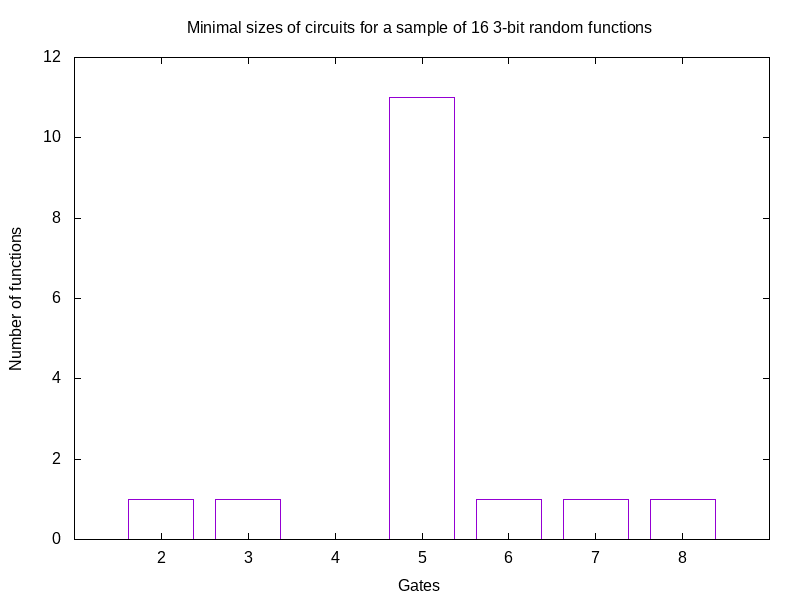
\includegraphics[width=\textwidth]{images/3rand_sizes.png}
  \label{fig:3rand_sizes}
  \caption{Sizes of optimal circuits for 3-bit functions with randomly chosen truth tables}
\end{figure}
\begin{figure}[!ht]
  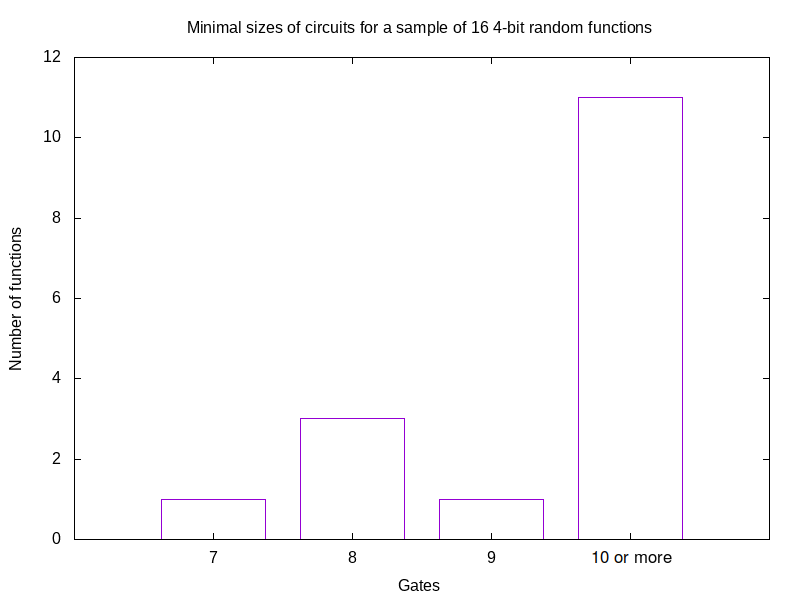
\includegraphics[width=\textwidth]{images/4rand_sizes.png}
  \label{fig:4rand_sizes}
  \caption{Sizes of optimal circuits for 4-bit functions with randomly chosen truth tables}

\end{figure}

A further 32 truth tables were generated for 4-bit inputs. While we expect a large proportion of circuits to be hard for large input sizes~\cite{arora}, the usual counting argument breaks down for such small values of n (ask for help - why?). However, using the SAT solver we can check the number of hard circuits directly.

*image*

\subsection{Extension axioms}

\section{Discussion}

\subsection{Reflection}

\subsection{Conclusions}

\subsection{Further directions}

\bibliographystyle{plain} 
\bibliography{sources}

\end{document}